%%%%%%%%%%%%%%%%%%%%%%% file rtree.tex %%%%%%%%%%%%%%%%%%%%%%
% Erweiterungen des R-Baums für räumliche Datenbankanfragen %
%%%%%%%%%%%%%%%%%%%%%%%%%%%%%%%%%%%%%%%%%%%%%%%%%%%%%%%%%%%%%


\documentclass[runningheads,a4paper]{llncs}

\usepackage{amssymb}
\setcounter{tocdepth}{2}
\usepackage{graphicx}
\graphicspath{ {./img/} }           % change graphics include path to ./img/

\usepackage[english, ngerman]{babel}
\usepackage[utf8]{inputenc}			    % for working umlaute
\usepackage[T1]{fontenc}            % wichtig fÃür Trennung von Wörtern mit Umlauten
\usepackage{microtype}						  % verbesserter Randausgleich
\usepackage{pdfpages}
\usepackage{lmodern}								%fuer schoenen Text in pdf-Abbildungen

\usepackage{array}
\usepackage{tabularx}								% for more convinient tables

\usepackage{quoting}
\usepackage[
	babel,
	german=quotes,
	threshold=2,										% two lines ore more triggers a blockquote
	thresholdtype=lines
]{csquotes}
% \SetBlockEnvironment{quoting}			% real block quotes
\renewcommand\mkblockquote[4]{\leavevmode\llap{„}#1#2#3“#4}			% block quotes with german quotation marks

% quellen mangement
\usepackage[
	backend=biber,
	natbib=true,								% damit \citep{} etc. verwendet werden können
	style=authoryear-icomp,    	% Zitierstil
	isbn=false,                	% ISBN nicht anzeigen, gleiches geht mit nahezu allen anderen Feldern
	pagetracker=true,          	% ebd. bei wiederholten Angaben (false=ausgeschaltet, page=Seite, spread=Doppelseite, true=automatisch)
	maxbibnames=10,            	% maximale Namen, die im Literaturverzeichnis angezeigt werden
	maxcitenames=2,            	% maximale Namen, die im Text angezeigt werden, ab 2 wird u.a. nach den ersten Autor angezeigt
	autocite=inline,           	% regelt Aussehen fÃür \autocite (inline=\parancite)
	block=space,               	% kleiner horizontaler Platz zwischen den Feldern
	backref=true,              	% Seiten anzeigen, auf denen die Referenz vorkommt
	backrefstyle=three+,       	% fasst Seiten zusammen, z.B. S. 2f, 6ff, 7-10
	date=short									% Datumsformat
]{biblatex}
\setlength{\bibitemsep}{0.6em}     	% Abstand zwischen den Literaturangaben
\setlength{\bibhang}{2em}        		% Einzug nach jeweils erster Zeile
% \renewcommand{\postnotedelim}{\addcolon\addspace}			% Doppelpunkt statt Komma vor der Seitenangabe in der Zitierung
% \DeclareFieldFormat{postnote}{#1}											% Kein einleitendes «S.» vor der Seitenangabe in der Zitierung

\bibliography{_literatur}

\usepackage[]{acronym}																% für Abkürzungen

\usepackage{hyperref}																	% for hyperlink references
\usepackage[ngerman, nameinlink]{cleveref}						% for naming references

\addto\extrasngerman{\def\figureautorefname{Abb.}}		% changes figure reference text to "Abb."

\usepackage{float}							        							% for use of "H" specifier in floats
\usepackage[section]{placeins}          							% keep floats (images, tables, ..) in their place

% change symbols for unordered lists (itemize)
\renewcommand{\labelitemi}{$\bullet$}
\renewcommand{\labelitemii}{$\circ$}


\begin{document}

\mainmatter  % start of an individual contribution

% first the title is needed
\title{Erweiterungen des R-Baums für räumliche Datenbankanfragen}

\subtitle{Der R*-Baum}

% a short form should be given in case it is too long for the running head
% \titlerunning{Verschiebungsalgorithmen für Kartenbeschriftungen}

\author{Patrick Schulz \& Simon Hötten}

% the affiliations are given next; don't give your e-mail address
% unless you accept that it will be published
\institute{Seminar Geodatenbanken \\ Dozent: Prof. Dr.-Ing. Jan-Henrik Haunert \\ Institut für Geoinformatik und Fernerkundung\\ Universität Osnabrück \\ Sommersemester 2015}

%\toctitle{Titel vom Inhaltsverzeichnis}
%\tocauthor{Authors' Instructions}
\maketitle
% Zusammenfassung
%%%%%%%%%%%%%%%%%%%%%%%%%%%%%%%%%%%%%%%%%%%%%%%%%%%%%%%%%%%%%%%%%%%%
% \begin{abstract}
\keywords{Geodatenbanken, R*, Spatial Access, Index, R-Tree}
% \end{abstract}


% Inhaltsverzeichnis
%%%%%%%%%%%%%%%%%%%%%%%%%%%%%%%%%%%%%%%%%%%%%%%%%%%%%%%%%%%%%%%%%%%%
% \tableofcontents
% \newpage


% Dokument
%%%%%%%%%%%%%%%%%%%%%%%%%%%%%%%%%%%%%%%%%%%%%%%%%%%%%%%%%%%%%%%%%%%%
\section{Motivation} % (fold)
\label{sec:intro}

	Herkömmliche eindimensionale Indexstrukturen bieten keine Möglichkeiten, mehrdimensionale räumliche Daten effizient zu durchsuchen. Die Reduzierung auf Punkte, um Objekte mit \ac{PAM} abzufragen, ist mit gewissen Einbußen möglich, aber insbesondere für komplexere Anfragen unzureichend.
	Der 1984 von Guttman entwickelte R-Baum \citep{Guttman:1984} versucht dieses Problem zu lösen, in dem der Index direkt auf den räumlichen Eigenschaften basiert. Mittlerweile existieren unzählige Varianten und Verwandte des R-Baums, dessen Einsatzgebiet weit über die klassische Geoinformatik hinaus geht.

	Eine dieser Varianten ist der R*-Baum, welcher die (teils unbegründeten) Annahmen in der ursprünglichen Veröffentlichung hinterfragt und so die Datenstruktur weiter optimiert. Im Folgenden gehen wir auf die Verfahren und Eigenheiten des regulären R-, als auch des R*-Baums ein, stellen allgemeine Optimierungskriterien auf und schließen mit einem Vergleich.

	Im Prinzip ist der R*-Baum für n-dimensionale Daten geeignet. Diese Arbeit beschränkt sich allerdings auf Geodaten, insbesondere sind alle Beispiele im zwei dimensionalen Raum. Hier liegt auch das Haupteinsatzgebiet von R*-Bäumen. Für höher-dimensionale Daten sind andere Indexstrukturen, wie der X-Baum, zu bevorzugen \citep[vgl.][28-29]{Kriegel:1996}.

% section intro (end)

\section{Prinzipien eines R-Baums} % (fold)
\label{sec:prinzipien_eines_r_baums}

Der R-Baum ist eine räumliche Indexstruktur für effiziente Bereichsabfragen von Geodaten im n-dimensionalen Raum. Der R-Baum teilt in jeder Ebene seiner Struktur die beinhalteten Geometrien der Geodaten in Partitionen auf. Die Gesamtheit der Geometrien einer Partitionen werden durch minimal umschließende Rechtecke (kurz \acs{MBR}) repräsentiert. 
Innerhalb einer Partition werden die Geoemtrien in weitere Partitionen unterteilt, bis die Anzahl der Geometrien den Schwellwert \acs{M} innerhalb einer Partition nicht mehr überschreitet. Der Vorteil dieser Strukturierung sorgt dafür, dass bei Bereichabfragen - zB. Was befindet sich in der Umgebung von Polygon p? - nicht zwingend alle Geometrien in der Ebene betrachtet werden müssen: Die \Cref{fig:beispiel-r-tree} stellt einen solchen R-Baum dar, wo bei einer Bereichsabfrage im besten Fall nach der ersten Entscheidungsebene die Hälfte des Geometriebestandes nicht mehr betrachtet werden muss. Wenn die \acs{MBR} einer Partition sich nicht in der Umgebung von Polygon p befindet, so werden auch alle darunterliegenden Ebenen der Partition nicht mehr behandelt. Die Verwendung von achsparallelen \acs{MBR} sorgt für effiziente Verschneidungs-Abfragen. Durch das alleinige Vergleichen der Koordinaten kann ermittelt werden, ob zwei \acs{MBR} sich schneiden oder nicht. Die Geometrien selbst werden ebenfalls durch \acs{MBR} repräsentiert, sind allerdings zur Bewahrung der Übersichtlichkeit in der \Cref{fig:beispiel-r-tree} nicht dargestellt.
\begin{figure}[H]
		\begin{center}
		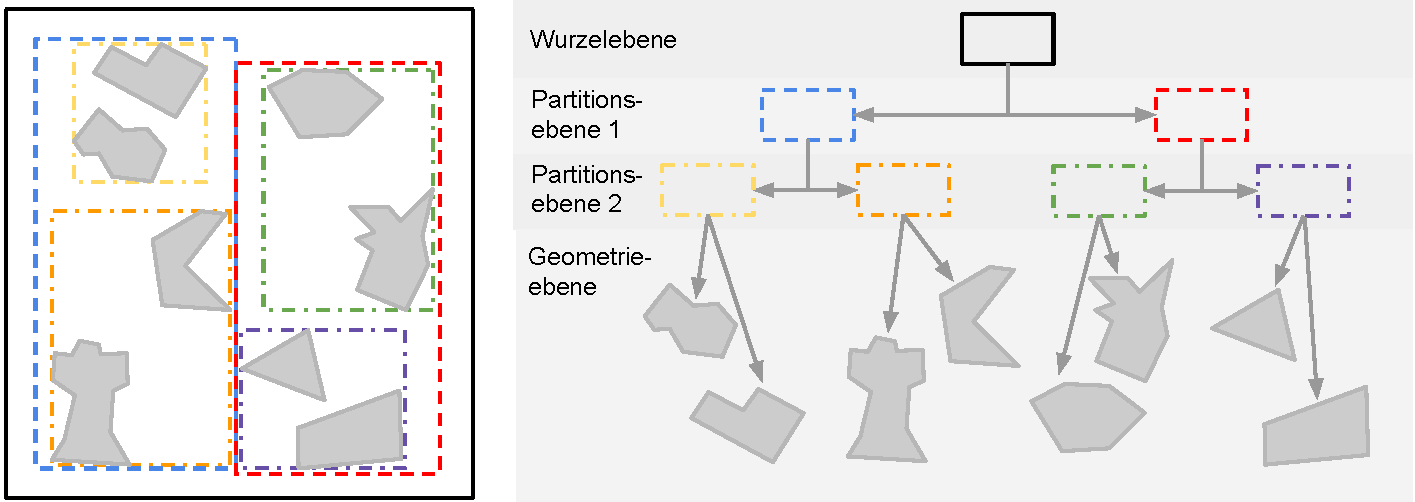
\includegraphics[width=1.0\textwidth ]{001_Beispiel_R-Tree.pdf}
		\caption{Beispiel für einen R-Baum. Links: Verteilung der Polygone und Partitionen im zweidimensionalen Raum. Rechts: Die dazugehörige Baumstruktur. (\acs{M}=3, \acs{m}=2)}
		\label{fig:beispiel-r-tree}
		\end{center}
	\end{figure}
Der Befüllen eines R-Baums verläuft iterativ, wo jedes einzelne Polygon separat nach einem Schema eingefügt wird. Der komplette Prozess des Einfügens lässt sich in zwei Methoden beschreiben, der Author bezeichnet diese Methoden als ChooseSubtree() und QuadraticSplit(). Beide Methoden werden in den nächsten Absätzen beschrieben. Abhängig in welcher Reihenfolge die Polygone in den R-Baum eingesetzt werden kommt es zu verschiedenen Verteilungen innerhalb des R-Baumes. Diese unterschiedlichen Verteilungsmöglichkeiten sind nicht immer ideal und sorgen für weniger effizientere Abfragen. Eie Neuverteilung der Polygone würde zu einer potenziell besseren Performance führen. Die Polygone in der \Cref{fig:beispiel-r-tree} sind im R-Baum zur Veranschaulichung ideal verteilt. Eine Lösung für dieses Problem wird in Kapitel \Cref{sec:rstar_reinsert} behandelt und ist Teil der Verbesserungen im R*-Baum.

\subsection{ChooseSubTree()}
\label{sec:r-choose-sub}
ChooseSubTree() ist eine rekursive Methode, die zu Beginn des Einfügevorgangs aufgerufen wird. Für die einzufügende Geometrie ist in der aktuellen Baum-Ebene die passende Partition zu finden, in dem die Goemetrie daraufhin zugeordnet werden soll. Der Vorgang wird in der darunterliegenden Ebene wiederholt bis die eigentliche Geometrie-Ebene erreicht wird. Bei der Auswahl der geeigneten Partition wird im R-Baum nur der potenzielle Flächenzuwachs des \acs{MBR} betrachtet. Die Geometrie wird der Partition zugewiesen, dessen \acs{MBR} den geringsten Flächenzuwachs erfährt. Lässt sich durch das erwähnte Kriterium kein eindeutiger Favorit ermitteln, wird danach entschieden, welches \acs{MBR} gesamtflächenmäßig kleiner ist. \Cref{fig:beispiel-choose-subtree} zeigt eine Situation in der untersten Baumebene mit zwei Partitionen, wo verglichen werden muss, welches der beiden Partitionen (rot oder blau) für das hellgraue Polygone am geeignetesten ist. Sobald die Geometrieebene erreicht wird, endet an dieser Stelle die ChooseSubTree()-Methode und die Geometrie wird in die erreichte Partition abgelegt. Abschließend wird überprüft, ob die neue Anzahl an Geometrien innerhalb der Partition den Wert \acs{M} überschritten hat. Wenn jenes der Fall ist, wird die QuadraticSplit()-Methode aufgerufen, ansonsten ist der Einfüge-Prozess abgeschlossen.

\begin{figure}[H]
		\begin{center}
		\includegraphics[width=1.0\textwidth ]{002_Beispiel_Choose_SubTree.pdf}
		\caption{ChooseSubTree()-Szenario. Links: Vergleich des Flächenzuwachses der Partitionen bei Aufnahme des Polygons. Rechts: hellgraues Polygon wird der blauen Partition zugeordnet, die den geringeren Flächenzuwachs erfährt. (\acs{M}=4, \acs{m}=2)}
		\label{fig:beispiel-choose-subtree}
		\end{center}
	\end{figure}

\subsection{QuadraticSplit()}
\label{sec:r-split}
Die QuadraticSplit() kümmert sich darum, dass überfüllte Partitionen nach dem Einfügen von Geometrien in zwei neue Partitionen aufgeteilt wird. Zuerst werden zwei Geometrien aus der Menge der Partition ermittelt, dessen \acs{MBR} den größten eindimensionalen Abstand voneinander aufweisen. In \Cref{fig:beispiel-quadratic-split} links ist das gesuchte Polygonpaar blau und grün markiert. Beide Polygone repräsentieren nun jeweils eine neue Partition. Abschließend werden die restlichen Polygone auf die beiden neuen Partitionen verteilt. Dabei kommt es zum selben Einfügeprozess, wie man es bereits von der ChooseSubTree()-Methode kennt. Die Reihenfolge, welches Polygon zuerst wieder eingefügt wird, wird durch die Differenz des potenziellen Flächenzuwachs der beiden neuen Partitionen ermittelt. Je höher die Differenz, desto früher wird das betroffene Polygon eingefügt. Da nach jedem Einfügevorgang werden die verbliebenen Polygone neu sortiert, da nach jedem Einfügen die erwähnte Differenz sich verändern kann. Wenn die Summe der verbliebenen Polygone und die Anzahl Polygone einer Partiotion den Wert \acs{m} ergibt, dann werden alle verbliebene Polygone der betroffenen Partition zugeordnet, um die Anforderung der Mindestpolygonanzahl \acs{m} zu erhalten und sich damit eine ungleichgewichtete Verteilung zwischen den beiden neuen Partitionen vermeiden lässt. Aus der Logik kann und darf die Variable \acs{m} nie größer \acs{M}/2 sein. Die beschriebene Zwangszuordnung ist ebenfalls eine Problemquelle für ungeschickte Zuordnungen. Nach der Verteilung der Geometrien auf die beiden neuen Partitionen wird abschließend in der nächsthöheren Partitionsebene auf eine Überfüllung überprüft. Der Splitvorgang propagiert sich nach oben und wird in der nächsthöhern Ebene ebenfalls durchgeführt, wenn die Partitionsauteilung in der vorherigen Ebene zu einer Überfüllung in der jetzigen Ebene geführt hat. 
\begin{figure}[H]
		\begin{center}
		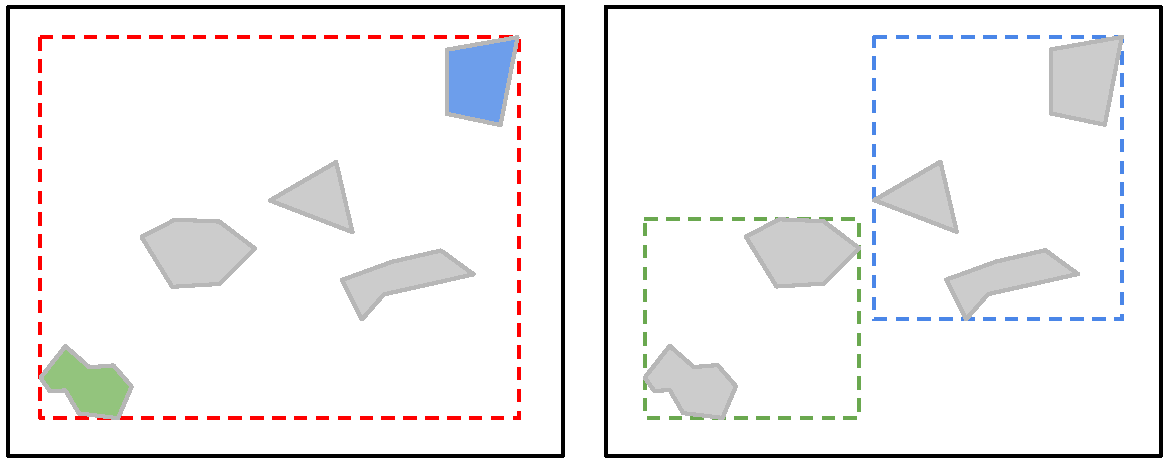
\includegraphics[width=1.0\textwidth ]{003_Beispiel_Quadratic_Split_1.pdf}
		\caption{Split()-Szenario. Links: Überfüllte Partition und gewähltes Polygonpaar, welche eine neue Partition repräsentieren. Rechts: Aufteilung der Polygone in die zwei neuen Partitionen. (\acs{M}=4, \acs{m}=2)}
		\label{fig:beispiel-quadratic-split}
		\end{center}
	\end{figure}

Der Grund, wieso die Methode QuadraticSplit() heißt und nicht einfach Split(), liegt daran, dass verschiedene Umsetzungen für die Aufteilung existieren, die eine Unterschiedliche Performance aufweisen. QuadraticSplit() deutet darauf hin, dass die Methode abhängig von der Anzahl Polygone eine quadratische Laufzeit besitzt. Neben dem QuadraticSplit() existieren noch der LinearSplit(), CubicSplit() und der GreenesSplit(). Der LinearSplit() unterscheidet sich vom QuadraticSplit() nur darin, dass dieser die Sortierung der ausstehenden Polygone nur einmal am Anfang durchführt. Dies sorgt zwar für eine bessere Laufzeit, die daraus resultierenden Aufteilungen werden im Vergleich zum QuadraticSplit() allerdings nie besser sein. (Aussage erwartet wahrscheinlich Beweis) Der CubicSplit hingegen verspricht, dass nach dem Flächenkriterium die besten Aufteilungen generiert wird auf Kosten der längeren Bearbeitungszeit. Der QuadraticSplit() ist somit ein Kompromiss zwischen Effizienz und Qualität. Dennoch gibt es Situationen, die zu ungünstigen Verteilungen führen. Ein markantes Beispiel ist in \Cref{fig:problem-tiny-object} dargestellt: Die Kombination von kleinen bzw. schmalen Geometrien, die zwar weit entfernt von einanderliegen und doch in ihrer Lage auf identischer Anhöhe liegen, sorgen für sehr schmale, nadelartige Partitionen, dessen \acs{MBR} mit einer sehr hohen Wahrscheilichkeit mit der anderen Partition überlappen.
\begin{figure}[H]
		\begin{center}
		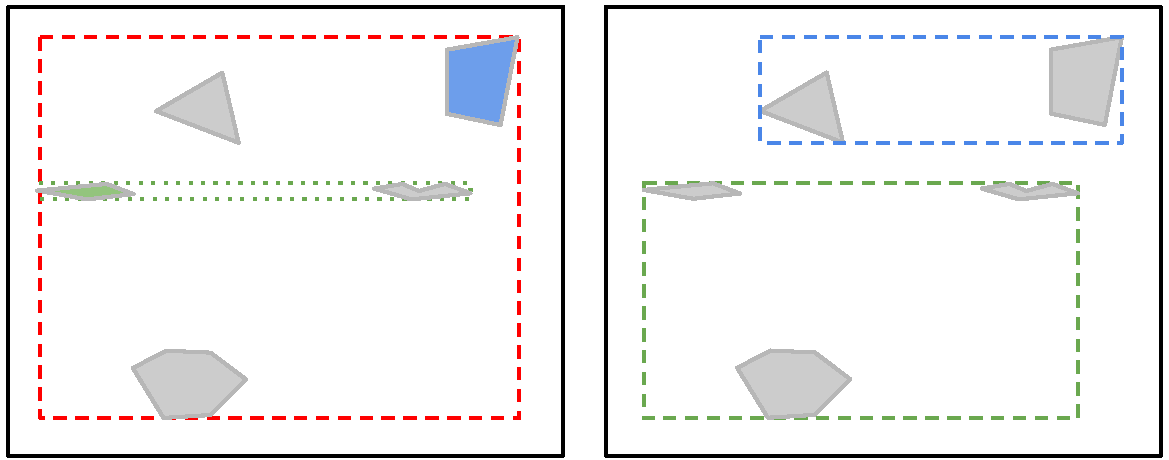
\includegraphics[width=1.0\textwidth ]{004_Problem_Kleine_Objekte.pdf}
		\caption{Problem der kleinen Objekte beim QuadraticSplit. Links: Durch die selbe Y-Achsen-Anhöhe zwischen den beiden schmalen Objekten entsteht ein sehr schmales \acs{MBR}. Rechts: Ergebnis des Splits auf Basis des initalen, schmalen \acs{MBR}s (\acs{M}=3, \acs{m}=2)}
		\label{fig:problem-tiny-object}
		\end{center}
	\end{figure} 

\subsection{GreenesSplit()}
\label{sec:grennes_split}
In einer der wissenschaftlichen Veröffentlichungen von "Greene" wird ein alternatives Verfahren für die bisher bekannten Split-Methoden vorgestellt. Die Idee besteht darin, die Polygone nach der jeweiligen Achse zu sortieren, in der die größte Ausbreitung ermittelt wird. Auf Basis dieser Sortierung hat man nun eine Reihe von möglichen Trenn-Lösungen, aus denen dann der Algorithmus den Favoriten ermittelt und übernimmt. Das Ergebniss in \Cref{fig:beispiel-greenes-split} rechts stellt den Favoriten dar mit der gerinsten Flächensumme. Man beachte, dass es zwei Möglichkeiten gibt, die Polygone nach einer Achse zu sortieren, nämlich nach ihrem Minimal- oder ihrem Maximalwert. In der \Cref{fig:beispiel-greenes-split} wird nur die Sortierung nach dem Minimalwert dargestellt. Bei der Wahl des Favoriten müssen die Trenn-Lösungen beider Sortierungen betrachtet werden. Neben dem besagten Flächenkriterium besitzt der GreenesSplit() im Vergleich zu den anderen Split-Algorithmen ein zusätzliches, geometrisches Kriterium: die Verteilung der Geometrien im Raum und die daraus ermittelte Trenn-Achse - wobei es auch hier zu Situationen kommen kann, in der sich der GreenesSplit() für die "falsche" Achse entscheidet. Es existieren allerdings noch weitere Kriterien, die im nächsten Kapitel aufgezählt werden, womit man die Verteilung im R-Baum optimieren könnte. 

\begin{figure}[H]
		\begin{center}
		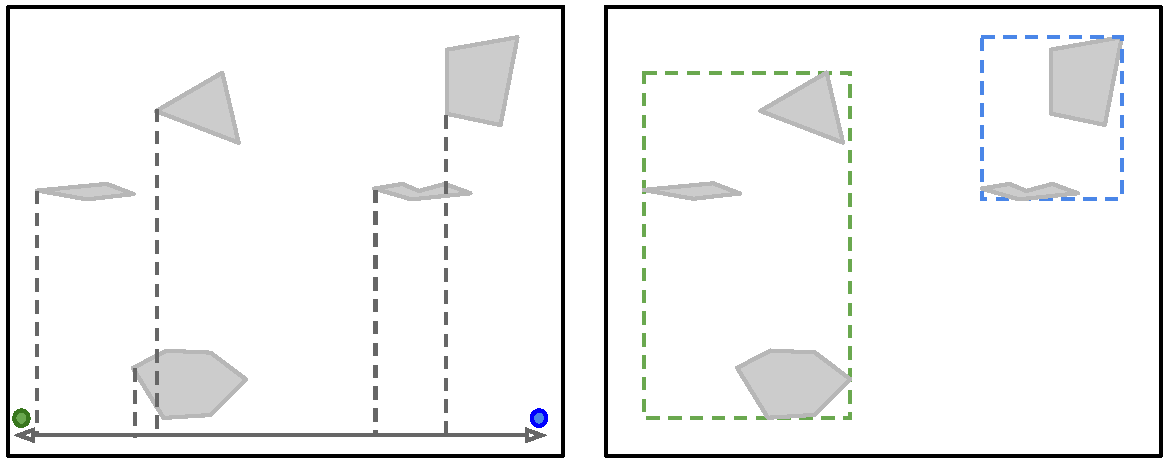
\includegraphics[width=1.0\textwidth ]{005_Beispiel_Greenes_Split.pdf}
		\caption{Beispiel für GreenesSplit. Links: Sortierung der Geometrien nach der gewählten Trenn-Achse. Rechts: Resultierende Ergebnis aus der Sortierung. (\acs{M}=3, \acs{m}=2)}
		\label{fig:beispiel-greenes-split}
		\end{center}
	\end{figure} 

% section prinzipien_eines_r_baums (end)

\section{Optimierungskriterien} % (fold)
\label{sec:optimierungskriterien}

	Bei dem herkömmlichen R-Baum wird, sowohl beim Hinzufügen neuer Elemente als auch beim Split, lediglich die Fläche der umschließenden Rechtecke minimiert \citep[vgl.][50-51]{Guttman:1984}. Einige der daraus resultierenden Probleme wurden bereits im vorherigen Abschnitt dargelegt.
	Im Folgenden werden weitere mögliche Optimierungen und ihre Wechselwirkungen aufgeführt. Ein R-Baum muss mit unterschiedlichen Geometrien und Anfragen umgehen können, daher wirken sich einige Kriterien in einigen Situationen stärker aus als andere.

	\subsubsection{Flächenausnutzung maximieren} % (fold)
	\label{ssub:flaechenausnutzung}

	Die Fläche, welche von dem umschließenden Rechteck, aber nicht von den in ihm enthaltenen Rechtecken, überdeckt wird, soll minimiert werden. Es soll also möglichst wenig Platz \enquote{verschwendet} werden. \citep[vgl.][323]{Beckmann:1990}

	% subsubsection flaechenausnutzung (end)

	\subsubsection{Überlappung minimieren} % (fold)
	\label{ssub:ueberlappung_minimieren}

	Die Überlappung der umschließenden Rechtecke soll minimiert werden. Dadurch müssen ebenfalls weniger Pfade im Baum traversiert werden. Liegt ein angefragter Punkt beispielsweise in einer Region, in der sich viele Rechtecke Überschneiden, müssen alle Möglichkeiten weiter verfolgt werden, was zu erhöhtem Rechenaufwand führt.
	
	% subsubsection ueberlappung_minimieren (end)

	\subsubsection{Summe der Kantenlänge minimieren} % (fold)
	\label{ssub:kantenlaenge}

	Die Summe der Kantenlänge der Verzeichnisrechtecke (\emph{\enquote{margin}}) soll möglichst klein sein. Quadrate werden also bevorzugt. Da Quadrate auf den jeweils höheren Ebenen im Baum besser zusammengefasst werden können, reduziert sich so die benötigte Fläche.
	Außerdem profitieren Anfragen mit großen, quadratischen Elementen von dieser Optimierung. \citep[vgl.][323]{Beckmann:1990}
	
	% subsubsection kantenlaenge (end)

	\subsubsection{Speichernutzung maximieren} % (fold)
	\label{ssub:speichernutzung_maximieren}

	Eine geringe Höhe des Baumes wirkt sich positiv auf die Kosten einer Abfrage aus. Das kann durch eine möglichst gleichmaßige Verteilung der Blattknoten erreicht werden. Insbesondere für große Abfragerechtecke ist dies relevant, da hier, auch abgesehen von den ersten drei genannten Optimierungen, mehrere Pfade traversiert werden müssen. \citep[vgl.][323-324]{Beckmann:1990}
	
	% subsubsection speichernutzung_maximieren (end)

	\subsubsection{Wechselwirkungen} % (fold)
	\label{ssub:wechselwirkungen}

	Um die Flächenausnutzung zu maximieren und die Überlappung zu minimieren, bedarf es einer größeren Freiheit bei der Wahl der Formen und der Anzahl an Rechtecken pro Knoten. Die Kriterien stehen also in Konkurrenz mit einer geringen Kantenlänge und hohen Speicherausnutzung. Auf der anderen Seite können quadratischere Rechtecke besser zusammengefasst werden, was sich wiederum positiv auf die Speichernutzung auswirkt. \citep[vgl.][323-324]{Beckmann:1990}
	
	% subsubsection wechselwirkungen (end)

% section optimierungskriterien (end)

\section{Der R*-Baum} % (fold)
\label{sec:rstar_tree}
In der bisher vorgestellten R-Baum-Variante war das einzigste Optimierungskriterium die Minierung der Flächeninhalte innerhalb der Partitionen. In \Cref{sec:optimierungskriterien} sind weitere potenzielle Kriterien gelistet, die während des Einfüge-Verfahrens berücksichtigt werden könnten. Diese besagten Kriterien wurden von den Authoren auf verschiedenste Weise kombiniert, untersucht und evaluiert. Dabei entstand aus den untersuchten Kombinationen die Methoden für den verbesserten R*-Baum, die auf Hinblick der Query-Performance die besten Ergebnisse liefern. \citep[vgl.][325]{Kriegel:2008}

\subsection{ChooseSubTree()}
Die ChooseSubTree()-Methode vom R*-Baum unterscheidet sich nicht erheblich von der bisher bekannten R-Baum-Variante. Der Unterschied zwischen den beiden rekursiven Methoden befindet sich im Entscheidungskriterium in der letzten Partitionsebene. Hier wird anstelle des Flächenkriteriums zuerst das Überlappungskriterium berücksichtigt. Der Grund, wieso nicht in allen Partitionsebenen nach dem Überlappungskriterium berücksichtigt werden, ist der Rechenaufwand, der für das Überpfüfen von Überlappungen benötigt wird. Der Aufwand ist quadratisch in Relation zu den vorhandenen Partitionen, zwischen denen gewählt werden muss. Im Falle einer hohen Anzahl von zu vergleichenden Partitionen steigt der Rechenaufwand erheblich. Für dieses Problem schlagen die Autoren vor, dass eine Vorauswahl der Partitionen stattfindet, in der nur die n-nächsten Partition als Kandidaten für die einzufügende Geometrie in Frage kommen. Determiniert werden diese Kandidaten durch das bisher bekannte Flächenkriterium. Anschließend wird nur "ungefähr" das Überlappungskriterium ermittelt, da hierfür nur die Überlappung zwischen den Kandidaten betrachtet wird. 

\subsection{Split()}
Die Split()-Methode besitzt die selbe Herangehensweise, wie der bereits erwähnte GreenesSplit() in \Cref{sec:grennes_split}. In beiden Methoden wird eine Trenn-Achse gewählt, die Partitionen sortiert und anschließend ein passender Split aus den Sortierungen gewählt. Der Unterschied liegt hierbei wieder in den Entscheidungskriterien. Bei der Wahl der Trenn-Achse wird für jede Achse die Menge aller Trenn-Lösungen aus den beiden bekannten Sortierungsmöglichkeiten erzeugt (siehe \Cref{fig:beispiel-trenn-loesungen}). Aus der Menge wird dann die Summe der Kantenlängen der Partitionen ermittelt. Als Trenn-Achse gewählt wird dann die Achse mit der geringsten Summe. Anschließend wird aus der gegebenen Lösungsmenge der Favorit ausgewählt, welche die geringste Überlappung zwischen den neuen Partitionen erzeugt. Ergibt sich durch die Betrachtung der Überlappung kein Favorit, wird bei einem Gleichstand die Lösung mit der geringeren Flächensumme ausgewählt. Das Problem der Überfüllung kann wie im R-Baum in die nächsthöhere Partitionsebene hochpropagieren, wo die Split()-Methode dann ggf. erneut ausgeführt wird.
\newline
Die Autoren haben neben den geometrischen Entscheidungskriterien auch mit Parametrisierung der Variablen \acs{M} und \acs{m} experimentiert und sind zu dem Ergebnis gekommen, dass die besten Splits entstehen, wenn \asc{m} ungefähr 40 Prozent von \acs{M} entspricht. \citep[vgl.][325]{Kriegel:2008}

	\begin{figure}[H]
		\centering
		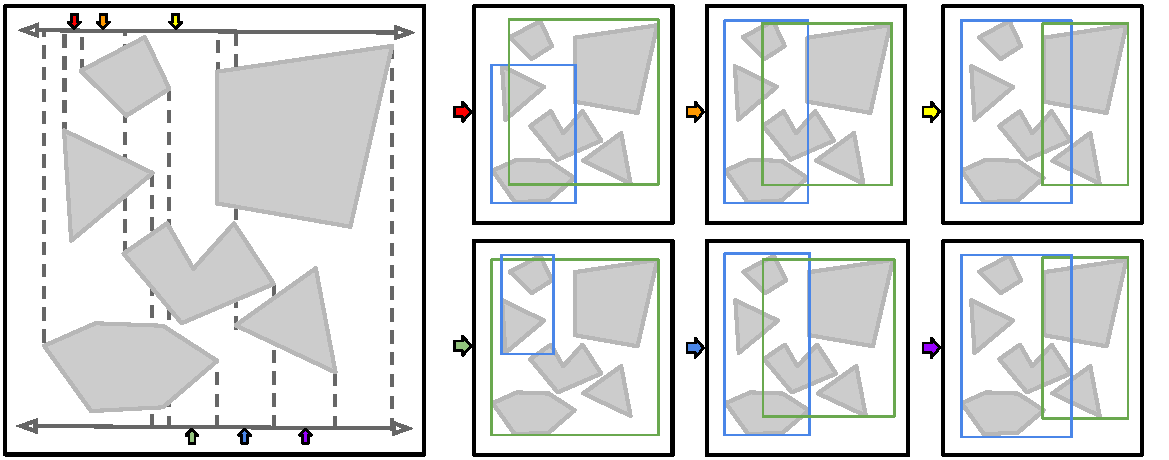
\includegraphics[width=1\textwidth]{006_Beispiel_Trenn_Loesungen.pdf}
		\caption{Aufzählung der Trenn-Lösungen für die waagerechte Achse. Die bunten Pfeile auf den grauen Sortierebene (links) verweisen auf die darausentstehenden Trenn-Lösungen. (\acs{M}=5, \acs{m}=2)}
		\label{fig:beispiel-trenn-loesungen}
	\end{figure}

\subsection{ForcedReinsert()}
\label{sec:rstar_reinsert}
Im \Cref{sec:prinzipien_eines_r_baums} ist das Problem des iterativen Einsetzverfahrens bereits angesprochen worden. Für dieses Problem ist der Ansatz einer Neu-Verteilung von gewählten Geometrien in die Baumstruktur eine natürliche Lösung um ungeschickte Verteilungen zu korrigieren, die durch eine ungünstige Einfügereihenfolge entstanden sind. Die Autoren bestätigen ihre Annahme durch einen Test, indem sie aus einem bestehenden, befüllten R-Baum die hälfte der Datensätze löschen und wieder in den Baum einfügen. Die daraus entstandene Struktur innerhalb vom R-Baum führte zu einer 50 Prozent verbesserten Query-Performance im Vergleich zur vorherigen Struktur \citep[vgl.][325]{Kriegel:2008}. Die ReInsert()-Methode wird nach jedem Einfügeprozess aufgerufen, sobald eine Partition überfüllt ist. Wenn die Methode das Überfüllungs-Problem nicht lösen konnte, wird erst dann die Split()-Funktion aufgerufen. Der Grund hierfür ist die Ambition solang wie möglich einen Split hinauszuzögern, welches ansonsten zu einer Propagierung des Überfüllungsproblems führen kann und dadurch  die Baum-Struktur unnötig erhöht werden kann. 
\newline
In der ReInsert()-Methode werden die beinhalteten \acs{MBR} der überfüllten Partition nach ihrer Zentralität sortiert. Die Zentralität definiert sich hier durch den Abstand zwischen dem Centroiden von dem \acs{MBR} und dem Centroiden von der überfüllten Partition. Basierend auf der Sortierung werden die \acs{p}-äußersten \ace{MBR} aus der Partition entfernt - dabei kann es sich sowohl um Geometrien, als auch um ganze Unter-Partitionen handeln. Anschließend werden die entfernten Objekte nach ihrer Sortierung entweder erst die Äußersten ("far reinsert") oder die inneren \acs{MBR} ("close reinsert") in die Struktur wieder eingefügt.
\newline
Durch verschiedene Tests empfehlen die Autoren für die Parametrisierung folgende Werte: Die Variable \acs{p} soll ungefähr 30 Prozent des beinhalteten Bestandes einer überfüllten Partition entsprechen und bei der Wiedereinfügereihenfolge sollte die "close reinsert"-Variante bevorzugt werden.

% section rstar_tree (end)

\section{Fazit} % (fold)
\label{sec:fazit}

	Zunächst lässt sich festhalten, dass der R*-Baum alle vorgestellten Optimierungskriterien berücksichtigt. Das hat einen etwas erhöhten Implementierungsaufwand gegenüber herkömmlichen R-Bäumen zur Folge.

	\begin{figure}[H]
		\centering
		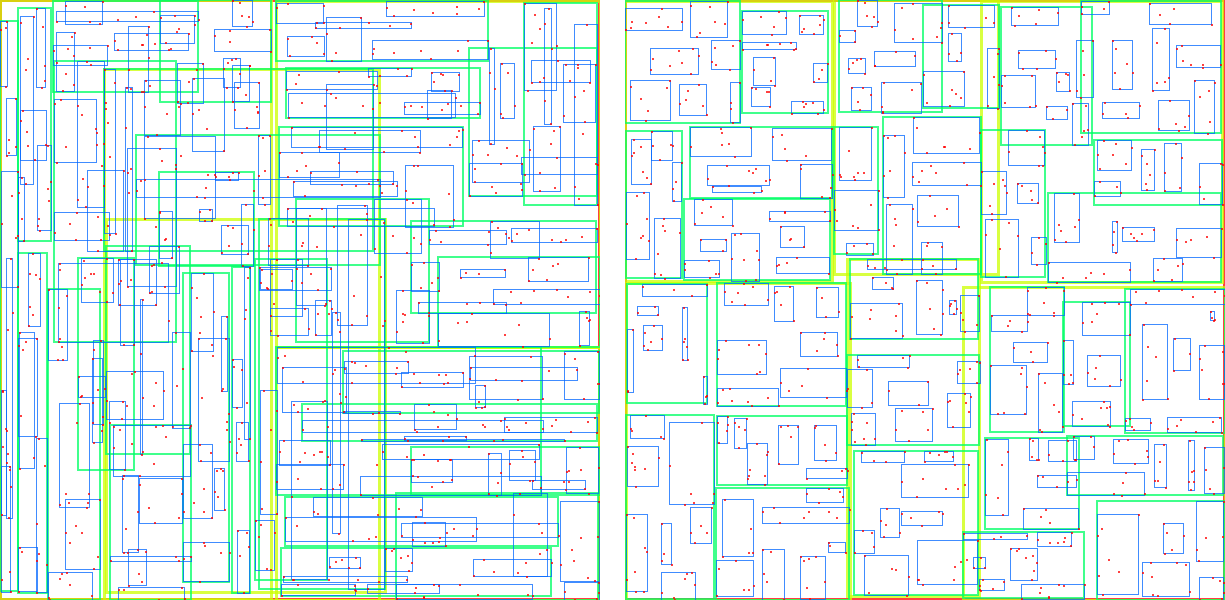
\includegraphics[width=1\textwidth]{vergleich-quad-star.png}
		\caption{Quadratischer- (links) und R*-Split (rechts) im Vergleich. (Bildquelle: \url{https://github.com/davidmoten/rtree})}
		\label{fig:vergleich-quad-star}
	\end{figure}

	Der R*-Baum betreibt sehr hohen Aufwand beim Hinzufügen und Löschen von Elementen, um eine gute Struktur zu bewahren. \Cref{fig:vergleich-quad-star} zeigt den gleichen Datensatz (mit gleicher Einfügereihenfolge), aber unterschiedlichen Split-Verfahren. Das Beispiel zeigt, wie positiv sich der Mehraufwand auswirkt. Mit R*-Split überschneiden sich die Verzeichnisrechtecke deutlich weniger, was schnellere Abfragen ermöglichen sollte und in den folgenden Benchmarks bestätigt wird.

	\subsubsection{Benchmarks} % (fold)
	\label{ssub:benchmarks}

	Die folgenden Benchmarks wurden von Beckmann, et.al. im Rahmen der ursprünglichen R*-Baum Veröffentlichung durchgeführt. Verglichen werden der originale R-Baum mit linearem, quadratischem und Greene-Split und der hier beschriebene R*-Baum. Die Parameter sind die für die jeweiligen Implementationen optimal gewählt\footnote{$m=20\%$ (von $M$ maximalen Einträgen) für den linearen Split, quadratischer Split: $m=40\%$, Greene's-Split: $m=40\%$ und R*-Split: $m=40\%$} \citep[vgl.][328]{Beckmann:1990}.

	Als Testdaten wurden fünf über verschiedene Verteilungen automatisch generierte Datensätze und ein realer Datensatz aus Höhenlinien gewählt (für eine genaue Beschreibung siehe \cite[328]{Beckmann:1990}). Die Daten wurden mit jeweils sieben verschiedenen Anfragen durchsucht und die Speicherzugriffe gemessen. Die Anfragen bestanden aus:
	\begin{description}
		\item[Point] Punkt-Anfrage ($1000\times$, gleich-verteilt im Raum)
		\item[Intersection] Suche nach allen Daten, welche die unterschiedlich großen Anfragerechtecke schneiden (je $100\times$, gleich-verteilt) (Größenangaben relativ zu der Größe des Testdatensatzes)
		\item[Contains] Suche nach allen Daten, die in den Anfragerechtecken komplett enthalten sind (ebenfalls je $100\times$, gleich-verteilt) (Größenangaben relativ zu der Größe des Testdatensatzes)
	\end{description}

	\begin{table}
	\caption{Vergleich der Bäume bei den verschiedenen Anfragen, gemittelt über die sechs Testdatensätze. Alle Angaben (bis auf Insert) sind relativ zu den Speicherzugriffen des R*-Baums. Insert zeigt die durchschnittlichen Speicherzugriffe beim Einfügen.}
	\label{tab:benchmark-queries}
	\begin{tabularx}{\textwidth}{l|X|X|X|X|X|X|X|X}
		& Point & \multicolumn{4}{c|}{Intersection} & \multicolumn{2}{c|}{Contains} & Insert \\
		& & $0.001\%$ & $0.01\%$ & $0.1\%$ & $1\%$ & $0.001\%$ & $0.01\%$ & \\
		\hline \hline
		linear	& $251.9$ & $242.2$ & $231.1$ & $189.8$ & $152.1$ & $256.5$ & $274.1$ & $12.63$	\\ \hline
		quad.		&	$135.3$ & $132.4$ & $132.8$ & $126.4$ & $117.6$ & $131.3$ & $137.0$ & $7.76$	\\ \hline
		Greene	& $148.7$ & $143.9$ & $148.0$ & $137.7$ & $121.3$ & $145.0$ & $155.2$ & $7.67$	\\ \hline
		R*			& $100$		& $100$		& $100$		& $100$		& $100$		& $100$		& $100$		& $6.13$
	\end{tabularx}
	\end{table}

	\begin{table}
	\caption{Performance der Bäume im Vergleich, hier gemittelt über alle sieben Anfragetypen. Alle Angaben sind relativ zu den Speicherzugriffen des R*-Baums.}
	\label{tab:benchmark-data}
	\begin{tabularx}{\textwidth}{l|X|X|X|X|X|X|X|X}
		& Gauß-Vert. & Cluster & Mix-Gleichvert. & Parzelliert & Höhenlinien & Gleichvert. \\
		\hline \hline
		linear	& $164.3$ & $216.0$ & $308.1$ & $247.2$ & $227.2$ & $206.6$	\\ \hline
		quad.		&	$112.9$ & $153.9$ & $121.8$ & $128.1$ & $144.5$ & $121.1$	\\ \hline
		Greene	& $123.1$ & $147.1$ & $115.5$ & $192.4$ & $144.2$ & $134.8$	\\ \hline
		R*			& $100$		& $100$		& $100$		& $100$		& $100$		& $100$
	\end{tabularx}
	\end{table}

	\Cref{tab:benchmark-queries} und \Cref{tab:benchmark-data} zeigen die, auf unterschiedliche Art aggregierten, Testergebnisse. Die bessere Performance des R*-Baums ist für alle verschiedenen Anfragen und Testdaten klar ersichtlich. Anzumerken ist, dass lediglich zwei dimensionale Daten verwendet wurden \citep[328][vgl.]{Beckmann:1990}. Das entspricht in den meisten Fällen den Anforderungen an Geodatenbanken. Für andere Anwendungsfälle wären weitere Tests notwendig.

	Interessant ist, dass trotz der Verwendung von Forced Reinsert der R*-Baum auch beim Einfügen von neuen Elementen schneller ist als herkömmliche Varianten.
	
	% subsubsection benchmarks (end)

	\subsubsection{Weiterentwicklungen} % (fold)
	\label{ssub:weiterentwicklungen}

	Die Effizienz des R*-Baums nimmt ab fünf Dimensionen rapide ab \citep[vgl.][29]{Kriegel:1996}. Um auch höher dimensionalen Daten gerecht zu werden, existieren daher zahlreiche Weiterentwicklungen. Dazu gehört, wie eingangs erwähnt, der X-Baum, welcher darauf ausgelegt ist auch in höheren Dimensionen Überlappungen zu vermeiden \citep[vgl.][]{Kriegel:1996}.
	Andere Indizes bilden Näherungen der tatsächlichen Daten und führen Anfragen zunächst auf diesen aus (\emph{\enquote{Vector Approximation}}, siehe \cite{Gibas:2008} oder \cite{Daoudi:2008}). So wird der Zugriff auf Daten mit über 100 Dimensionen vergleichsweise effizient ermöglicht \citep[vgl.][]{Daoudi:2008}.
	
	% subsubsection weiterentwicklungen (end)

% section fazit (end)



% Anhang
%%%%%%%%%%%%%%%%%%%%%%%%%%%%%%%%%%%%%%%%%%%%%%%%%%%%%%%%%%%%%%%%%%%%
\newpage
\begin{appendix}

	\section*{Anhang}
	\addcontentsline{toc}{section}{Anhang}

	\section*{Abkürzungsverzeichnis} % (fold)
	\label{sub:abbreviations}

		\begin{acronym}[length]
			\acro{m}{Variable: minimale Anzahl der Geometrien in einer Partition}
			\acro{M}{Variable: maximale Anzahl der Geometrien in einer Partition}
			\acro{p}{Variable: Anzahl der zu entfernenden Geometrien/Partitionen in der ReInsert()-Methode}
			\acro{MBR}{Minimum bounding Rectangle}
		  \acro{SAM}{Spatial access methods}
		  \acro{PAM}{Point access methods}
	  \end{acronym}

	% section abbreviations (end)

	% Abbildungsverzeichnis
	% \listoffigures

	% Literaturverzeichnis
	%%%%%%%%%%%%%%%%%%%%%%%%%%%%%%%%%%%%%%%%%%%%%%%%%%%%%%%%%%%%%%%%%%%%b
	\nocite{*}							% include all bibtex entries from bibliography, even if they are not citied in the document

	\printbibliography

\end{appendix}

\end{document}
